\documentclass[a4paper,11pt]{article}
%================================================================================================================================================================
% Preamble
%================================================================================================================================================================
\usepackage{lscape}
\usepackage{a4wide}		%wider margins for a4 paper
\usepackage{amssymb}
\usepackage{amsmath}
\usepackage{graphicx}
\usepackage{url}
\usepackage{hyperref}	%automatic links to sections, figures, references
\usepackage[all]{hypcap}%links to top of figures
\usepackage{soul}		%highlighting with \hl{}
\usepackage{color}		%color, also color highlighting
\usepackage{xcolor}
\usepackage{setspace}	%line spacing
\usepackage{multirow}	%multirow and multicolumn cells in tables
\usepackage{subfig}		%\subfloat in figures
\usepackage{multicol}
\usepackage{paracol}
%\usepackage[version=3]{mhchem}		%\ce{} for chemical formulae
\usepackage{wrapfig}	%\begin{wrapfigure}
\usepackage{lscape}
\usepackage{enumerate}
\usepackage[toc,page]{appendix}
\usepackage[final]{pdfpages}
\usepackage{amsfonts}              % for blackboard bold, etc
\usepackage{amsthm}                % better theorem environments
\usepackage{tabularx}
\usepackage{array}
\usepackage{listings} 
\usepackage{enumerate,letltxmacro}
\usepackage[none]{hyphenat}


\usepackage{fancyhdr}
\pagestyle{fancy}
\fancyhead[R]{MCB 5430 final}
\fancyhead[L]{Bianca Mocanu}
\cfoot{\thepage}

%================================================================================================================================================================

\usepackage{Sweave}
\begin{document}
\Sconcordance{concordance:Final.tex:Final.Rnw:%
1 43 1 1 0 45 1 1 4 3 0 1 1 1 4 2 0 1 1 11 0 1 1 1 5 3 0 1 6 4 0 3 1 5 %
0 1 1 4 0 1 2 1 7 6 0 1 2 3 1 5 0 1 1 4 0 1 2 7 1 1 2 1 0 1 1 1 3 2 0 1 %
4 13 0 1 9 7 0 1 5 3 0 1 2 5 0 1 3 13 0 1 1 10 0 1 2 1 4 3 0 1 1 5 0 2 %
1 9 0 1 4 7 0 2 1 1 2 8 0 1 3 6 0 1 3 7 0 2 2 1 0 1 2 6 0 1 1 1 2 6 0 1 %
3 2 0 1 1 11 0 2 1 11 0 1 3 2 0 1 2 7 0 1 2 5 1 1 2 1 0 4 2 9 0 1 2 5 0 %
2 2 5 0 1 3 1 0 4 1 4 0 1 2 8 1 1 7 6 0 1 3 1 0 1 1 1 2 5 0 1 2 1 4 3 0 %
1 4 3 0 2 1 4 0 1 2 6 1 1 2 1 0 1 3 1 0 1 2 1 3 1 0 1 2 5 0 1 2 1 1 1 2 %
5 0 1 1 5 0 1 2 2 1 1 7 5 0 1 3 1 0 1 3 1 0 1 3 1 0 1 3 1 0 1 3 1 0 1 2 %
9 0 1 2 21 1 1 2 1 0 1 1 1 2 1 1 1 2 5 0 1 4 2 0 2 2 8 0 1 2 5 0 1 3 1 %
2 1 0 1 2 11 0 3 2 18 0 1 2 32 0 1 4 1 0 1 5 3 0 1 2 6 0 1 2 5 0 1 2 1 %
5 76 0 1 2 34 1 1 4 3 0 1 2 18 0 1 4 2 0 1 2 1 0 1 2 1 0 1 6 4 0 1 2 1 %
3 2 0 3 2 1 5 3 0 2 2 4 0 1 3 3 1 1 2 1 0 2 1 1 4 2 0 1 1 1 3 2 0 1 1 1 %
3 2 0 2 1 1 5 9 0 1 3 4 1 1 2 1 0 2 1 1 2 1 4 6 0 1 2 44 1}


%================================================================================================================================================================

\title{MCB 5430 final assignment}
\author{Bianca Mocanu}

%================================================================================================================================================================
% Title page
%================================================================================================================================================================
\begin{titlepage}

\begin{center}
\noindent \Large{\textbf{MCB 5430 final assignment}}\\
\vspace{0.7cm}
\small{Bianca Mocanu}\\
\today
\end{center}

%================================================================================================================================================================
\tableofcontents
\end{titlepage}
%================================================================================================================================================================

\section{RNA-seq processing}

\subsection{Pipeline for RNAseq data and generating bedgraph files}

The RNA-seq processing script can be also found \href{https://github.com/biancamocanu/5430_RNAseq/blob/master/pipe.sh}{\color{blue}here\color{black}}. It has the following steps:\\

\begin{itemize}
\item{fastqc analysis of the initial fastq files provided on the server}
\item{quality trimming of the fastq files and fastqc analysis of the output}
\item{alignment using HISAT2}
\item{bedgraph files generation for UCSC (with header) and with no header}
\item{stringtie read quantification}
\item{prepDE.py for edgeR compatible tables}
\item{logfile}

\end{itemize}

\subsection{Comparison of replicates}
First, the csv document from prepDE is imported as a matrix in R. A quick look at the matrix shows that to access the values for the E2 replicates, we need the first two columns, and to access the untreated replicates, we need columns 3 and 4.
The log2 scatterplots can then be obtained by using the plot function with X and Y values as the log2 of the 1st and 2nd column values, respectively, for E2. Likewise, the 3rd and 4th columns are used to plot the same thing for untreated:

\begin{Schunk}
\begin{Sinput}
> #Starting prepDE counts files are in this directory:
> 
> directory="~/5430_RNAseq/prepDE/"
> setwd(directory)
> # Importing the csv file gene_count_matrix 
> 
> countData <- as.matrix(read.csv("gene_count_matrix.csv", row.names="gene_id"))
> head(countData)
\end{Sinput}
\begin{Soutput}
                   E2_rep1 E2_rep2 untr_rep1 untr_rep2
ENSG00000116032.5        8      13        11        15
ENSG00000137288.5      574     395       622       426
ENSG00000167578.12     394     326       187       288
ENSG00000102081.9     1338    1341      1794      1713
ENSG00000167531.2        0       1         0         1
ENSG00000103227.14     635     452      1150       514
\end{Soutput}
\begin{Sinput}
> dfcountData <- data.frame(countData)
> plot(log2(dfcountData[,1]), log2(dfcountData[,2]), pch=20, col='gray60',
+      cex=0.2, main="Log2 scatterplot of the E2 replicates", 
+      xlab="Log2(E2 rep 1 counts)", 
+      ylab="Log2(E2 rep 2 counts)")
> # When adding the fit line and finding the correlation, there is a problem 
> # for genes whose counts are zero. To fix this, I added 0.1 to the counts
> # number for those commands (does not alter the countData matrix).
> 
> model1 <- lm(log2(dfcountData[,1]+0.1) ~ log2(dfcountData[,2]+0.1))
> abline(model1, col="red")
> model1_cor <- cor(log2(dfcountData[,1]+0.1), log2(dfcountData[,2]+0.1))
> model1_cor
\end{Sinput}
\begin{Soutput}
[1] 0.9703333
\end{Soutput}
\begin{Sinput}
> text(14, 1, paste("R squared =", round(model1_cor, digits=4)))
\end{Sinput}
\end{Schunk}
\includegraphics{Final-001}

\begin{Schunk}
\begin{Sinput}
> # Same for the untreated replicates 1 and 2:
> 
> plot(log2(dfcountData[,3]), log2(dfcountData[,4]), pch=20, col='gray60',
+      cex=0.2, main="Log2 scatterplot of the untreated replicates", 
+      xlab="Log2(untr_rep 1 counts)",
+      ylab="Log2(untr_rep 2 counts)")
> model2 <- lm(log2(dfcountData[,3]+0.1) ~ log2(dfcountData[,4]+0.1))
> abline(model2, col="red")
> model2_cor <- cor(log2(dfcountData[,3]+0.1), log2(dfcountData[,4]+0.1))
> model2_cor
\end{Sinput}
\begin{Soutput}
[1] 0.9642606
\end{Soutput}
\begin{Sinput}
> text(14, 1, paste("R squared =", round(model2_cor, digits=4)))
\end{Sinput}
\end{Schunk}
\includegraphics{Final-002}


\section{Differential Gene Expression Analysis}
\subsection{EdgeR quantification of differences between datasets}
For the EdgeR step, a multi dimensional DGEList object must be created. The DGEList function that creates the object requires as input the matrix and a "group" object that, in this case, groups the datasets based on whether they are the untreated controls or the treated samples.\\
In order to identify differentially expressed genes as accurately as possible, transcripts with very low counts are being excluded, as they are more error-prone. Here, only the genes having more than one read per million in 3 out of 4 samples are being kept. Next, the data is normalized and the common and tagwise dispersions and variance values are calculated (tagwise, as required by the final exam questions). According to the results below, overall each data point can vary up to about 25 percent between replicates. The tagwise variance values are for each individual data point (here, 12719 of them).\\
The DE genes are called using the tagwise dispersion model, and the resulting table is filtered to keep entries with FDR values below 0.05. The remaining data from the remaining 394 genes can then later be highlighted in MA and MDS plots (see next sections). 

\begin{Schunk}
\begin{Sinput}
> library(edgeR)
> library(car)
> # Get the name of the columns for the samples
> 
> sampleNames <- colnames(countData)
> # Take a look at how countData object is displayed
> 
> head(countData)
\end{Sinput}
\begin{Soutput}
                   E2_rep1 E2_rep2 untr_rep1 untr_rep2
ENSG00000116032.5        8      13        11        15
ENSG00000137288.5      574     395       622       426
ENSG00000167578.12     394     326       187       288
ENSG00000102081.9     1338    1341      1794      1713
ENSG00000167531.2        0       1         0         1
ENSG00000103227.14     635     452      1150       514
\end{Soutput}
\begin{Sinput}
> # Creating groups (all samples that are untreated, all samples that are
> # treated) to be used for DGEList object later. The group syntax is such
> # that you name the label for the first group and then how many columns
> # are grouped, then same for 2nd group. Must be in that order that you 
> # see in head(countData). Here, first two columns are the treated ones,
> # next 2 columns are teh untreated ones.
> 
> groups=c(rep("treated",2), rep('untreated',2))
> # DGEList function creates the DGEList object for the edgeR. We call it
> # cds here
> 
> cds <- DGEList(countData, group=groups)
> names(cds)   # this displays the components of the cds object
\end{Sinput}
\begin{Soutput}
[1] "counts"  "samples"
\end{Soutput}
\begin{Sinput}
> # the cds object right now has the dataset with the counts and also some
> # information about the groups of samples that you have
> head(cds$counts)
\end{Sinput}
\begin{Soutput}
                   E2_rep1 E2_rep2 untr_rep1 untr_rep2
ENSG00000116032.5        8      13        11        15
ENSG00000137288.5      574     395       622       426
ENSG00000167578.12     394     326       187       288
ENSG00000102081.9     1338    1341      1794      1713
ENSG00000167531.2        0       1         0         1
ENSG00000103227.14     635     452      1150       514
\end{Soutput}
\begin{Sinput}
> head(cds$samples)
\end{Sinput}
\begin{Soutput}
              group lib.size norm.factors
E2_rep1     treated 20671047            1
E2_rep2     treated 17738490            1
untr_rep1 untreated 17051619            1
untr_rep2 untreated 15544963            1
\end{Soutput}
\end{Schunk}

\begin{Schunk}
\begin{Sinput}
> # Filtering poorly expressed genes
> cds <- cds[rowSums(1e+06 * cds$counts/expandAsMatrix(cds$samples$lib.size,
+                             dim(cds)) > 1) >=3, ]
> dim(cds)
\end{Sinput}
\begin{Soutput}
[1] 12719     4
\end{Soutput}
\begin{Sinput}
> cds <- calcNormFactors(cds)
> cds$samples
\end{Sinput}
\begin{Soutput}
              group lib.size norm.factors
E2_rep1     treated 20671047    0.9819417
E2_rep2     treated 17738490    0.9814447
untr_rep1 untreated 17051619    1.0163386
untr_rep2 untreated 15544963    1.0209631
\end{Soutput}
\begin{Sinput}
> #Effective library sizes after normalization
> 
> cds$samples$lib.size * cds$samples$norm.factors
\end{Sinput}
\begin{Soutput}
[1] 20297762 17409348 17330218 15870834
\end{Soutput}
\begin{Sinput}
> cds <- estimateCommonDisp(cds)
> cds <- estimateTagwiseDisp(cds, prior.df = 10)
> names(cds) # now cds has much more info than before
\end{Sinput}
\begin{Soutput}
 [1] "counts"             "samples"            "common.dispersion" 
 [4] "pseudo.counts"      "pseudo.lib.size"    "AveLogCPM"         
 [7] "prior.df"           "prior.n"            "tagwise.dispersion"
[10] "span"              
\end{Soutput}
\begin{Sinput}
> # View common dispersion
> cds$common.dispersion
\end{Sinput}
\begin{Soutput}
[1] 0.06696863
\end{Soutput}
\begin{Sinput}
> # View tagwise dispersion values for several datapoints
> head(cds$tagwise.dispersion)
\end{Sinput}
\begin{Soutput}
[1] 0.05933810 0.08756400 0.02700631 0.06424450 0.11769392 0.07335725
\end{Soutput}
\end{Schunk}

\begin{Schunk}
\begin{Sinput}
> tag_variance <- sqrt(as.numeric(cds$tagwise.dispersion))
> # View tagwise variance values for several datapoints
> head(tag_variance)
\end{Sinput}
\begin{Soutput}
[1] 0.2435941 0.2959121 0.1643360 0.2534650 0.3430655 0.2708454
\end{Soutput}
\begin{Sinput}
> common_variance <- sqrt(as.numeric(cds$common.dispersion))
> # View overall variance
> common_variance
\end{Sinput}
\begin{Soutput}
[1] 0.258783
\end{Soutput}
\begin{Sinput}
> # Using tagwise dispersion model to call significantly changed genes
> de.tgw <- exactTest(cds, dispersion = cds$tagwise.dispersion, 
+                     pair = c("untreated", "treated"))
> head(de.tgw$table)
\end{Sinput}
\begin{Soutput}
                        logFC   logCPM     PValue
ENSG00000137288.5  -0.2994285 4.834848 0.40563805
ENSG00000167578.12  0.3988901 4.077626 0.36762094
ENSG00000102081.9  -0.5650186 6.470863 0.01919016
ENSG00000103227.14 -0.7864615 5.289378 0.03545942
ENSG00000188385.7  -0.1026021 2.148375 0.85714033
ENSG00000078237.4  -0.4883074 4.198229 0.22446361
\end{Soutput}
\begin{Sinput}
> resultsTbl.tgw <- topTags(de.tgw, n=nrow(de.tgw$table))$table
> head(resultsTbl.tgw)
\end{Sinput}
\begin{Soutput}
                       logFC   logCPM       PValue          FDR
ENSG00000145439.7  -4.164982 6.645059 9.548435e-44 1.214465e-39
ENSG00000164626.8   4.733557 5.137123 9.437399e-35 6.001714e-31
ENSG00000136997.10  3.061029 7.457766 1.212849e-32 5.142077e-29
ENSG00000146243.9   4.714053 5.548333 8.016414e-31 2.549019e-27
ENSG00000113739.6   2.734506 8.182189 5.915024e-30 1.504664e-26
ENSG00000164128.2   3.805286 5.407338 1.262955e-28 2.677254e-25
\end{Soutput}
\begin{Sinput}
> #Creating new table with significantly changed genes - here entries with
> # FDR values above 0.05 are being discarded
> de.genes.tbl.tgw <- resultsTbl.tgw[ resultsTbl.tgw$FDR <= 0.05, ]
> # This displays how many genes have FDR <= 0.05
> dim(de.genes.tbl.tgw)
\end{Sinput}
\begin{Soutput}
[1] 394   4
\end{Soutput}
\end{Schunk}

\subsection{PCA plot}
The PCA plot, just like the MDS plot, can display the relationship between samples. They differ slightly in the way they define the "distance" between samples. As per the final exam request, this subsection shows the steps for a PCA plot. Despite previous analysis being done using EdgeR, DEseq2 package can build an object that can be then modified and used as an argument of DEseq2's plotPCA function, as seen below. At this point, the R environment already has the colData matrix from previous commands. The res object is somewhat equivalent to EdgeR's de.genes table that has been filtered for the FDR 0.05 upper threshold.\\

The PCA plot here considers the two most informative dimensions to show how the samples differ from each other. For example, on the X axis (1st PC), the untreated samples are very close to each other, which can be interpreted as a high degree of similarity, while the treated ones are a bit farther from each other.\\

\begin{Schunk}
\begin{Sinput}
> library(DESeq2)
> condition <- c( "treated", "treated", "untreated","untreated")
> colData <- data.frame(condition)
> row.names(colData) <- sampleNames
> colData
\end{Sinput}
\begin{Soutput}
          condition
E2_rep1     treated
E2_rep2     treated
untr_rep1 untreated
untr_rep2 untreated
\end{Soutput}
\begin{Sinput}
> all(rownames(sampleNames) %in% colnames(countData))
\end{Sinput}
\begin{Soutput}
[1] TRUE
\end{Soutput}
\begin{Sinput}
> countData <- countData[, sampleNames]
> all(rownames(colData) == colnames(countData))
\end{Sinput}
\begin{Soutput}
[1] TRUE
\end{Soutput}
\begin{Sinput}
> dds <- DESeqDataSetFromMatrix(countData = countData, colData = colData,
+                               design = ~ condition)
> dds<- DESeq(dds)
> res <- results(dds, alpha=0.05)
> rld <- rlogTransformation(dds, blind=TRUE)
> plotPCA(rld, intgroup=c('condition'))
\end{Sinput}
\end{Schunk}
\includegraphics{Final-006}

\subsection{MA plot}
For the MA plot, two approaches are possible: either using a standard plot function or edgeR's integrated plotSmear function.\\

For the simple plot function, the log of the Fold Change can be plotted against the total counts per million from the initial output dataset of edgeR (resultsTbl.tgw). Then, we can overlay this plot with the same log of the Fold Change against the total counts per million from the filtered dataset (for the FDR $<=$ 0.05) and display these data points e.g. in red, to show which of these genes are significantly changed. For guidance, horizontal lines for y = 1 and -1 can be included which, on the log2 Y axis, indicate where a fold change of 2 and $1/2$, respectively, would be.\\

One observation here is that some genes can be confidently called as being differentially expressed even though their change is less than doubled, when upregulated, or less than halved, when downregulated. This is possible because the total counts per million are high enough so that the result is more confident than for low expressed genes.


\begin{Schunk}
\begin{Sinput}
> # The MA plot using plot function
> 
> plot(resultsTbl.tgw$logCPM, resultsTbl.tgw$logFC, pch=20, col='grey60',
+      cex=0.5,main = "Tagwise dispersion MA plot using plot() and points()",
+      xlab="log2(total CPM)", 
+      ylab="log2(Fold Change)")
> # adding horizontal lines for y = -1 and 1
> abline(h=-1, lty=5)
> abline(h=1, lty=5)
> points(de.genes.tbl.tgw$logCPM, de.genes.tbl.tgw$logFC, pch=20, col='red',
+        cex=0.75)
\end{Sinput}
\end{Schunk}
\includegraphics{Final-007}

\begin{Schunk}
\begin{Sinput}
> # The MA plot using EdgeR's plotSmear function
> 
> de.genes.tgw <- rownames(resultsTbl.tgw)[resultsTbl.tgw$FDR <= 0.05]
> plotSmear(cds, de.tags=de.genes.tgw, 
+           main="Tagwise dispersion MA plot using plotSmear", 
+           pair=c("untreated", "treated"), cex=0.35, xlab="log CPM", 
+           ylab="Log fold-change")
> abline(h=-1, lty=2)
> abline(h=1, lty=2)
\end{Sinput}
\end{Schunk}
\includegraphics{Final-008}

\subsection{Up and down-regulated genes}

To obtain the up and downregulated gene name lists, the starting point is the output file of EdgeR, resultsTbl.tgw.\\
The upregulated and downregulated genes are defined as entries with the FDR value $<=$ 0.05 which have logFC values above zero or below zero, respectively. These entries, however, have row names that correspond to the transcript variants of the genes, as indicated by the number after the separating ".".
To reach to the gene name alone, a splitting function must be applied to all rows of the Up and Downregulated genes list.

\begin{Schunk}
\begin{Sinput}
> library(rtracklayer)
> write.table(resultsTbl.tgw , file="all_genes_tgw.txt", col.names =T, 
+             row.names=T)
> resultsTbl.tgw <- read.table("all_genes_tgw.txt")
> #filter based on FDR
> de.genes.tgw <- resultsTbl.tgw[ resultsTbl.tgw$FDR <= 0.05,]
> dim(de.genes.tgw)
\end{Sinput}
\begin{Soutput}
[1] 394   4
\end{Soutput}
\begin{Sinput}
> E2_up <- de.genes.tgw [de.genes.tgw $logFC >0,]
> E2_down <- de.genes.tgw [de.genes.tgw $logFC <0,]
> dim(E2_up)
\end{Sinput}
\begin{Soutput}
[1] 280   4
\end{Soutput}
\begin{Sinput}
> dim(E2_down)
\end{Sinput}
\begin{Soutput}
[1] 114   4
\end{Soutput}
\begin{Sinput}
> Genes.all <- rownames(resultsTbl.tgw)
> E2_up_names <- rownames(E2_up)
> E2_down_names <- rownames(E2_down)
> # The above gene names still have the transcript variant attached after
> # the "." separator. In order to obtain
> # The gene name, they need to be split:
> 
> Genes.all_split <- sapply(Genes.all, function(x) 
+   unlist(strsplit(x, split="[.]"))[1])
> E2up_split <-sapply(E2_up_names, function(x) 
+   unlist(strsplit(x, split="[.]"))[1])
> E2down_split <-sapply(E2_down_names, function(x) 
+   unlist(strsplit(x, split="[.]"))[1])
> write.table(as.data.frame(Genes.all_split), file="Genes_all_split.txt",
+             row.names=TRUE, col.names=TRUE)
> write.table(as.data.frame(E2up_split), file="E2_upregulated_split.txt", 
+             row.names=TRUE, col.names=TRUE)
> write.table(as.data.frame(E2down_split), file="E2_downregulated_split.txt", 
+             row.names=TRUE, col.names=TRUE)
> head(Genes.all_split)
\end{Sinput}
\begin{Soutput}
 ENSG00000145439.7  ENSG00000164626.8 ENSG00000136997.10  ENSG00000146243.9 
 "ENSG00000145439"  "ENSG00000164626"  "ENSG00000136997"  "ENSG00000146243" 
 ENSG00000113739.6  ENSG00000164128.2 
 "ENSG00000113739"  "ENSG00000164128" 
\end{Soutput}
\end{Schunk}

Following the sapply function, however, the lists and text files still contain the initial gene name (with "."), as well as the gene name. An easy fix is using the following commands in the terminal to cut this space delimited text, remove the "" surrounding gene names and retrieve only the gene names, and eventually remove the precursor text file.

\begin{verbatim}
cat Genes_all_split.txt | cut -d " " -f2 |  sed 's/[^a-z  A-Z 0-9]//g'
  > Gene_names_all.txt 

# rm Genes_all_split.txt

cat E2_upregulated_split.txt | cut -d " " -f2 | sed 's/[^a-z  A-Z 0-9]
//g'  > Upregulated_names.txt

# rm E2_upregulated_split.txt

cat E2_downregulated_split.txt | cut -d " " -f2 | sed 's/[^a-z  A-Z 0-9]
//g' > Downregulated_names.txt

# rm E2_downregulated_split.txt
\end{verbatim}

\subsection{Gene Ontology analysis using GOseq}

\begin{Schunk}
\begin{Sinput}
> library(goseq)
> library(org.Hs.eg.db)
> up.vector=as.integer(Genes.all_split%in%E2up_split)
> down.vector=as.integer(Genes.all_split%in%E2down_split)
> head(up.vector)
\end{Sinput}
\begin{Soutput}
[1] 0 1 1 1 1 1
\end{Soutput}
\begin{Sinput}
> # Add names from all genes to vector
> 
> names(up.vector)<-Genes.all_split
> names(down.vector)<-Genes.all_split
> head(up.vector)
\end{Sinput}
\begin{Soutput}
ENSG00000145439 ENSG00000164626 ENSG00000136997 ENSG00000146243 ENSG00000113739 
              0               1               1               1               1 
ENSG00000164128 
              1 
\end{Soutput}
\begin{Sinput}
> pwf_up=nullp(up.vector,"hg19","ensGene")
> 
\end{Sinput}
\end{Schunk}
\includegraphics{Final-010}

\begin{Schunk}
\begin{Sinput}
> pwf_down=nullp(down.vector,"hg19","ensGene")
> head(pwf_up)
\end{Sinput}
\begin{Soutput}
                DEgenes bias.data        pwf
ENSG00000145439       0      2128 0.01996940
ENSG00000164626       1      3787 0.02889231
ENSG00000136997       1      1346 0.01456005
ENSG00000146243       1      1161 0.01314117
ENSG00000113739       1      5347 0.02983885
ENSG00000164128       1      2762 0.02423019
\end{Soutput}
\begin{Sinput}
> GO.wall_up=goseq(pwf_up,"hg19","ensGene", method = "Wallenius")
> GO.wall_down=goseq(pwf_down,"hg19","ensGene", method = "Wallenius")
> head(GO.wall_up)
\end{Sinput}
\begin{Soutput}
        category over_represented_pvalue under_represented_pvalue numDEInCat
4484  GO:0010604            3.312885e-07                1.0000000         80
4299  GO:0009893            1.809705e-06                0.9999994         82
12191 GO:0048534            1.920803e-06                0.9999994         29
17418 GO:1902107            4.554821e-06                0.9999994         10
1026  GO:0002520            6.967464e-06                0.9999976         29
18068 GO:1903708            8.658716e-06                0.9999987         11
      numInCat                                                   term ontology
4484      2044 positive regulation of macromolecule metabolic process       BP
4299      2183               positive regulation of metabolic process       BP
12191      461            hematopoietic or lymphoid organ development       BP
17418       70       positive regulation of leukocyte differentiation       BP
1026       492                              immune system development       BP
18068       91                     positive regulation of hemopoiesis       BP
\end{Soutput}
\begin{Sinput}
> head(GO.wall_down)
\end{Sinput}
\begin{Soutput}
        category over_represented_pvalue under_represented_pvalue numDEInCat
3367  GO:0007179            2.198142e-05                0.9999975          8
15201 GO:0071560            8.446198e-05                0.9999883          8
15200 GO:0071559            8.897599e-05                0.9999876          8
10067 GO:0042704            1.095039e-04                1.0000000          2
3366  GO:0007178            1.097169e-04                0.9999818          9
6784  GO:0030278            1.266944e-04                0.9999844          7
      numInCat
3367       128
15201      155
15200      156
10067        2
3366       204
6784       123
                                                                          term
3367                transforming growth factor beta receptor signaling pathway
15201            cellular response to transforming growth factor beta stimulus
15200                              response to transforming growth factor beta
10067                                                   uterine wall breakdown
3366  transmembrane receptor protein serine/threonine kinase signaling pathway
6784                                                regulation of ossification
      ontology
3367        BP
15201       BP
15200       BP
10067       BP
3366        BP
6784        BP
\end{Soutput}
\begin{Sinput}
> enriched.GO.BP_up=GO.wall_up$category[
+   p.adjust(GO.wall_up$over_represented_pvalue, method="BH")<0.05]
> #The FDR of 0.01 would not give many results here, so I had to use 0.05 and worse.
> 
> enriched.GO.BP_down=GO.wall_down$category[
+   p.adjust(GO.wall_down$over_represented_pvalue, method="BH")<0.1]
> head(enriched.GO.BP_up)
\end{Sinput}
\begin{Soutput}
[1] "GO:0010604" "GO:0009893" "GO:0048534" "GO:1902107" "GO:0002520"
[6] "GO:1903708"
\end{Soutput}
\begin{Sinput}
> head(enriched.GO.BP_down)
\end{Sinput}
\begin{Soutput}
character(0)
\end{Soutput}
\begin{Sinput}
> library(GO.db)
> for(go in enriched.GO.BP_up[1:5]){
+ print(GOTERM[[go]])
+ cat("--------------------------------------\n")
+ }
\end{Sinput}
\begin{Soutput}
GOID: GO:0010604
Term: positive regulation of macromolecule metabolic process
Ontology: BP
Definition: Any process that increases the frequency, rate or extent of
    the chemical reactions and pathways involving macromolecules, any
    molecule of high relative molecular mass, the structure of which
    essentially comprises the multiple repetition of units derived,
    actually or conceptually, from molecules of low relative molecular
    mass.
--------------------------------------
GOID: GO:0009893
Term: positive regulation of metabolic process
Ontology: BP
Definition: Any process that activates or increases the frequency, rate
    or extent of the chemical reactions and pathways within a cell or
    an organism.
Synonym: activation of metabolic process
Synonym: positive regulation of metabolism
Synonym: stimulation of metabolic process
Synonym: up regulation of metabolic process
Synonym: up-regulation of metabolic process
Synonym: upregulation of metabolic process
--------------------------------------
GOID: GO:0048534
Term: hematopoietic or lymphoid organ development
Ontology: BP
Definition: The process whose specific outcome is the progression of
    any organ involved in hematopoiesis (also known as hemopoiesis) or
    lymphoid cell activation over time, from its formation to the
    mature structure. Such development includes differentiation of
    resident cell types (stromal cells) and of migratory cell types
    dependent on the unique microenvironment afforded by the organ for
    their proper differentiation.
Synonym: haematopoietic or lymphoid organ development
Synonym: haemopoietic or lymphoid organ development
Synonym: hemopoietic or lymphoid organ development
--------------------------------------
GOID: GO:1902107
Term: positive regulation of leukocyte differentiation
Ontology: BP
Definition: Any process that activates or increases the frequency, rate
    or extent of leukocyte differentiation.
Synonym: activation of immune cell differentiation
Synonym: activation of leucocyte differentiation
Synonym: activation of leukocyte differentiation
Synonym: positive regulation of immune cell differentiation
Synonym: positive regulation of leucocyte differentiation
Synonym: up regulation of immune cell differentiation
Synonym: up regulation of leucocyte differentiation
Synonym: up regulation of leukocyte differentiation
Synonym: up-regulation of immune cell differentiation
Synonym: up-regulation of leucocyte differentiation
Synonym: up-regulation of leukocyte differentiation
Synonym: upregulation of immune cell differentiation
Synonym: upregulation of leucocyte differentiation
Synonym: upregulation of leukocyte differentiation
--------------------------------------
GOID: GO:0002520
Term: immune system development
Ontology: BP
Definition: The process whose specific outcome is the progression of an
    organismal system whose objective is to provide calibrated
    responses by an organism to a potential internal or invasive
    threat, over time, from its formation to the mature structure. A
    system is a regularly interacting or interdependent group of organs
    or tissues that work together to carry out a given biological
    process.
--------------------------------------
\end{Soutput}
\end{Schunk}


\section{Comparison of regulated genes with ChIP-seq data}
\subsection{Bedtools for distances between ChIP peaks and nearest gene TSSs}
To calculate these distances, the following steps need to be done and considered:

\begin{itemize}
\item Use bedtools closest to report the distances between the summits (-a) and gene TSSs (-b) with respect to the TSS positions (-D b).
\item To be able to plot this information later, only one TSS must be printed in the event of a tie (-t first)
\item To get the TSSs, start with a bed file with all the genes and reformat it (e.g. using awk) so that the transcription start site is either the 2nd or 3rd column in the bed file, depending on the strand where the gene is.
\item I don't think there is a need for further processing like flanking the TSSs by e.g. 50 nucleotides each way, since bedtools closest reports only one distance from a summit to the closest TSS
\item Since further analysis asks for comparison with the up, down, and non-regulated genes, the gene names must be the Ensemble IDs "ENSG[...]" in order to be compatible with the text files with all the genes retrieved in Part 2, section 4.
\end{itemize}

\begin{verbatim}
awk '{if($6=="+")
> printf ("%s\t%s\t%s\t%s\t%s\t%s\n", $1, $2, $2, $4, $5, $6);
> else
> printf ("%s\t%s\t%s\t%s\t%s\t%s\n", $1, $3, $3, $4, $5, $6)
> }' hg19_gencode_ENSG_geneID.bed > hg19_gencode_TSS_ENSG_geneID.bed
\end{verbatim}

The file with the TSS then needs to be sorted. The sorted file can be used with bedtools closest with the -D b and -t first options:\\

\begin{verbatim}
bedtools sort -i hg19_gencode_TSS_ENSG_geneID.bed > 
                            hg19_gencode_TSS_ENSG_geneID_sorted.bed

rm hg19_gencode_TSS_ENSG_geneID.bed

bedtools closest -D b -t first -a /tempdata3/MCB5430/final_data/ER_peaks
/ER_E2_summits.bed -b hg19_gencode_TSS_ENSG_geneID_sorted.bed > 
                                                ER_E2_closest_all.bed
\end{verbatim}

\begin{Schunk}
\begin{Sinput}
> #loading the BED file into R
> E2_all_closest <- read.table("ER_E2_closest_all.bed", 
+               header=FALSE, sep="\t", stringsAsFactors = FALSE)
> head(E2_all_closest)
\end{Sinput}
\begin{Soutput}
    V1      V2      V3          V4  V5   V6      V7      V8              V9 V10
1 chr1  856576  856577 MACS_peak_1   7 chr1  860259  860259 ENSG00000187634 591
2 chr1 1009194 1009195 MACS_peak_2 125 chr1 1009687 1009687 ENSG00000237330 592
3 chr1 1014951 1014952 MACS_peak_3  33 chr1 1009687 1009687 ENSG00000237330 592
4 chr1 1316033 1316034 MACS_peak_4  12 chr1 1310875 1310875 ENSG00000175756  74
5 chr1 1368560 1368561 MACS_peak_5  25 chr1 1370240 1370240 ENSG00000179403 595
6 chr1 2379468 2379469 MACS_peak_6  10 chr1 2357418 2357418 ENSG00000149527  75
  V11   V12
1   + -3682
2   -   492
3   - -5264
4   - -5158
5   + -1679
6   + 22050
\end{Soutput}
\begin{Sinput}
> #loading the lists of names in R
> all_gene_names <- read.table("Gene_names_all.txt", header=TRUE, 
+               stringsAsFactors = FALSE)
> upreg_names <- read.table("Upregulated_names_sorted.txt", 
+               header=TRUE, stringsAsFactors = FALSE)
> downreg_names <- read.table("Downregulated_names_sorted.txt", 
+               header=TRUE, stringsAsFactors = FALSE)
> # To subset the E2_all_closest, I first selected the rows on the
> # condition that V9 (the ENSG name) is within the gene list names, then
> # picked those rows from E2_all_closest
> 
> selected_rows <- (E2_all_closest$V9 %in% upreg_names$E2upsplit) 
> Upreg_closest <- E2_all_closest[selected_rows,] 
> #this is the dataframe with only upregulated genes
> 
> selected_rows <- (E2_all_closest$V9 %in% downreg_names$E2downsplit) 
> Downreg_closest <- E2_all_closest[selected_rows,] 
> selected_rows <- (E2_all_closest$V9 %in% all_gene_names$Genesallsplit)
> Allgenes_closest <- E2_all_closest[selected_rows,]
> # To obtain the non-regulated table, I then removed the regulated genes
> # rows from the E2_all_closest dataset 
> 
> library(dplyr)
> Regulated_closest <- union(Upreg_closest, Downreg_closest)
> Nonregulated_closest <- setdiff(Allgenes_closest, Regulated_closest)
> 
\end{Sinput}
\end{Schunk}

\subsection{CDF plot}
The cumulative distribution plots shown here allow to estimate how far from the TSS most of the ChIP peaks are. The X axis is for the distance between the TSS and the ChIP peaks and the y axis shows what proportion of peaks are within x basepairs from the TSS. The bedtools closest generated distances that have + and -, so in order to make meaningful plots, the absolute value of the reported distance is used here.

\begin{Schunk}
\begin{Sinput}
> up_closest_cdf <- ecdf(abs(Upreg_closest[,12]))
> down_closest_cdf <- ecdf(abs(Downreg_closest[,12]))
> non_closest_cdf <- ecdf(abs(Nonregulated_closest[,12]))
> plot(up_closest_cdf, xlim=c(0,50000), ylim=c(0.1, 0.9), 
+      col="forestgreen", main = "CDF plot of ER E2 distance to TSS", 
+      xlab="Distance (bps)", ylab = "Fraction", las=1)
> par(new=TRUE)
> plot(down_closest_cdf, xlim=c(0,50000), ylim=c(0.1, 0.9), 
+      col="red", main = "CDF plot of ER E2 distance to TSS", 
+      xlab="Distance (bps)", ylab = "Fraction", las=1)
> par(new=TRUE)
> plot(non_closest_cdf, xlim=c(0,50000), ylim=c(0.1, 0.9), 
+      col="black", main = "CDF plot of ER E2 distance to TSS", 
+      xlab="Distance (bps)", ylab = "Fraction", las=1)                       
> abline(h=0.5, lty=2)
> abline(h=0.2, lty=2)
> legend( x="topleft", legend=c("Upregulated genes",
+                                   "Downregulated genes", 
+                                   "Non-regulated genes"), 
+         col=c("forestgreen","red", "black"), lwd=1, lty=c(1,1,1), 
+         pch=c(NA,NA) )
> 
\end{Sinput}
\end{Schunk}
\includegraphics{Final-013}

\subsection{Box plots}

The starting point for boxplots are the Upreg\_closest, Downreg\_closest and Nonregulated\_.closest. These are currently dataframes that all have 12 variables and different number of rows (observations). Combining these separate datasets by columns doesn't work well (or serve the purpose), as they all have different number of rows. To be able to use combine them so that the boxplots are plotted together, I'd create a new column for each of these three, containing the type of effect ER has on the genes (upregulating, downregulating, or none), combine the tables with this new column, and plot the distances grouped by the effect.

\begin{Schunk}
\begin{Sinput}
> Upreg_closest$effect<-"Upregulated"
> Downreg_closest$effect<-"Downregulated"
> Nonregulated_closest$effect<-"Nonregulated"
> Genes_with_effects<- rbind(Upreg_closest, Downreg_closest, Nonregulated_closest)
> boxplot(abs(Genes_with_effects$V12) ~ Genes_with_effects$effect, outline=F, 
+         border=c("red", "grey40", "forestgreen"),
+         main="Distribution of distances between ChIP peaks and gene TSS", lty=1)
\end{Sinput}
\end{Schunk}
\includegraphics{Final-014}


\subsection{The nature of the mechanism of gene activation / repression by ER}

According to the CDF plot, only approximately 20 percent of peaks are less than 10k basepairs away from the TSS for upregulated genes. For non-regulated genes and downregulated genes, it seems even worse.\\
The boxplots reveal the same thing, as the peaks for downregulated genes seem to be much farther away from gene TSS than for non-regulated and upregulated genes, as well as much more dispersed.\\
These results are expected for the estrogen receptor, given the previous ChIP seq analyses done for the midterm which showed that this receptor has a very strong preference for enhancers and binds very little to TSS. This is not consistent with what I would expect for a canonical transcription factor (such as ATF1). I would think that a transcription factor prefers areas around gene TSS and binds directly to those, which would result in a very steep CDF line that would look asymptotic at a much higher fraction (much closer to 1), within 50000 basepairs. The boxplots would also look much more condensed.   

\subsection{UCSC Browser shot}

To find an upregulated gene on Chromosome 12, I used the following commands:

\begin{verbatim}
cat Upregulated_names.txt | while read line
> do
> grep $line hg19_gencode_ENSG_geneID.bed >> upgenesssss.bed
> done
\end{verbatim}

\begin{verbatim}
chr12   119616446       119632551       ENSG00000152137 1497    +
chr12   123468026       123594975       ENSG00000090975 190     -
chr12   31433517        31479050        ENSG00000139146 12      -
chr12   116396380       116715143       ENSG00000123066 184     -
chr12   76419226        76425384        ENSG00000139289 1168    -
chr12   64238072        64541613        ENSG00000196935 134     +
chr12   2904118 2913124 ENSG00000004478 607     +
\end{verbatim}

The second gene in the list above is displayed in the attached browser shot. Its RefSeq name is PITPNM2.\\

\section{Bonus question - cat hairball DNA motif}

For the catball motif, I thought I could run blat or bwa on the GGGGGCCCCCAT sequence, get the coordinates, subtract or add 904,100 to the coordinates and then see what motifs can lie around.
BWA and Blat seem to consider this sequence too short to allow that (they want at least 50 basepairs), so I uploaded the hairball dna text file as a fasta file in Benchling and I searched for the GGGGGCCCCCAT as a motif there - I found it to be at 3074588-3074599, which means the motif we are looking for is around position 2170488-2170499, as shown below:

\begin{center}
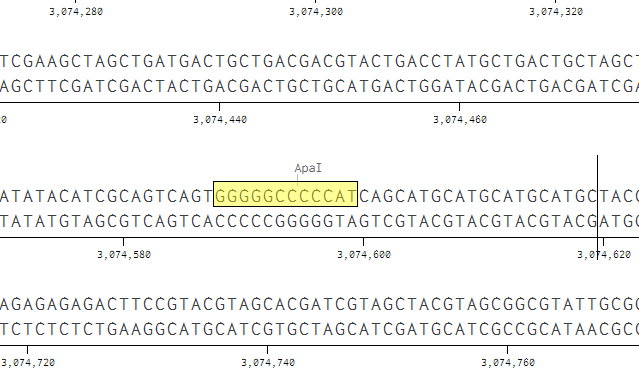
\includegraphics{ss0.png}
\hline
\hline
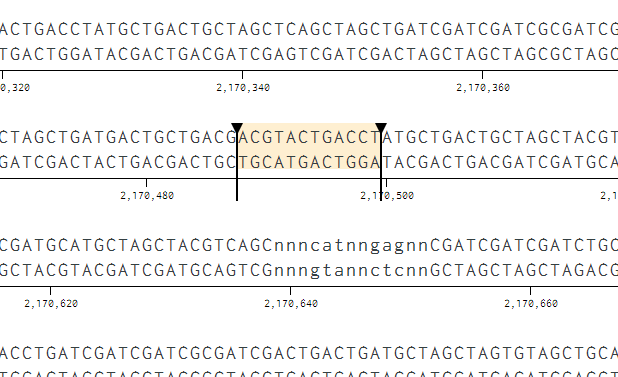
\includegraphics{ss1.png}
\end{center}

The best guess is that the motif is therefore within the sequence TGCATGACTGGA. Could as well be longer or shorter, but the answer for this is "CATGAC" because it did make me sigh audibly.
\end{document}
